\documentclass[10pt,a4paper]{article}
\usepackage[utf8]{inputenc}
\usepackage[spanish]{babel}
\usepackage{amsmath}
\usepackage{amsfonts}
\usepackage{amssymb}
\usepackage{graphicx}
\usepackage{multicol}
\usepackage{titling}
\usepackage{titlesec}
\usepackage{array}
\usepackage{bm}
\usepackage{afterpage}
\usepackage{float}
\usepackage{graphicx}
\usepackage{epstopdf}
\usepackage{longtable}
\usepackage{xcolor}
\usepackage{epigraph}
\setlength\epigraphwidth{1.5\textwidth}
\usepackage{subfigure}
\usepackage{anyfontsize}
\usepackage[left=2cm,right=2cm,top=2cm,bottom=2cm]{geometry}
\usepackage[colorlinks=true,
            linkcolor=blue,
            citecolor=blue,
            urlcolor=blue]{hyperref}

\begin{document}
\author{Lisseth C. Alban-Checa} % CAMBIAR A AUTORES
\title{MATERIA DE SISTEMAS MICROPROCESADOS\\ % TITULO  \\ ES ENTER
LABORATORIO PUERTOS DIGITALES Y COMUNICACION SERIAL}
\maketitle  
\section{Introducción} % nuevas secciones
\begin{multicols}{2} % texto en 2 colomnas
La mayoría de los pines de los microcontroladores son multipropósito, es decir, en función de su configuración se comportan de una forma u otra. \\
El ATmega328p como cualquier otro microcontrolador tiene registros, algunos de estos registros están conectados con los puertos de entrada/salida, cada puerto tiene un nombre específico y sus registros asociados, de hecho, el 328p tiene los puertos B, C y D, y cada puerto 8 pines de la MCU conectados. En función del encapsulado puede haber una restricción en el número de pines. Por ejemplo en el paquete de 28 pines PDIP. \\
La comunicación serial es muy importante porque gran parte de los protocolos utilizados actualmente son serie y además muchos dispositivos de comunicación inalámbrica usan la comunicación serie para hablar con Arduino como los módulos bluetooth y los módulos Xbee. También la comunicación serie es la que se usa generalmente para comunicar el Arduino con el Ordenador.
\end{multicols} %termina texto en columnas
\section{Diseño del Sistema}
\subsection{Diagrama de Flujo}
Ingresar su diagrama de flujo realizado en cualquier programa.
\begin{figure}[ht!]
\caption{Diagrama de flujo} % ingresa nombre de la figura (caption)
\centering
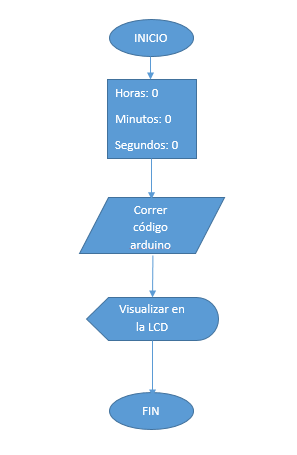
\includegraphics[scale=0.6]{DIAGRAMA DE FLUJO.png} % cambie el valor de la escala entre 0.1-1 para el tamano de la misma
\end{figure}\\ %termina figura y envia enter
Ingrese su diagrama de bloques
\begin{figure}[hbt!]
\caption{Diagrama de bloques} % ingresa nombre de la figura (caption)
\centering
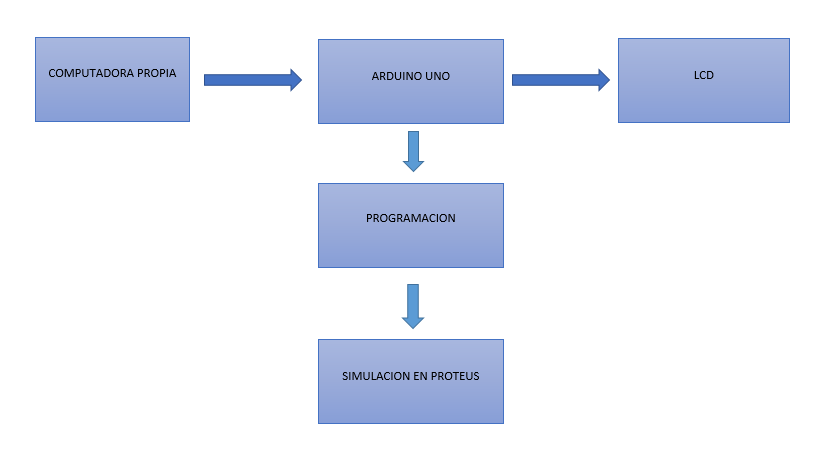
\includegraphics[scale=0.5]{DIAGRAMA DE BLOQUES.png}
\end{figure}

\section{Desarrollo}

\subsection{Simulación}
Ingrese su simulación

\begin{figure}[ht!]
\caption{Simulacion en proteus}
\centering
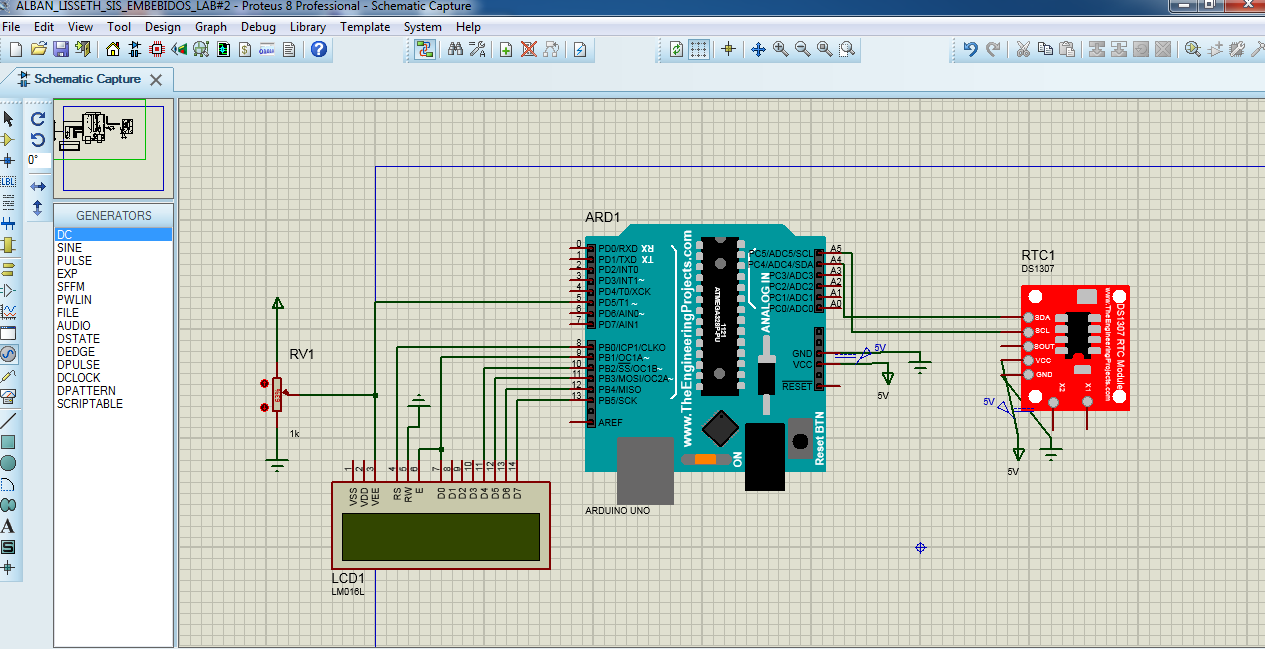
\includegraphics[scale=0.3]{SIMULACION.png}
\end{figure} 

Ingrese su armado en fritzing 
\begin{figure}[hbtp]
\caption{Armado del sistema}
\centering
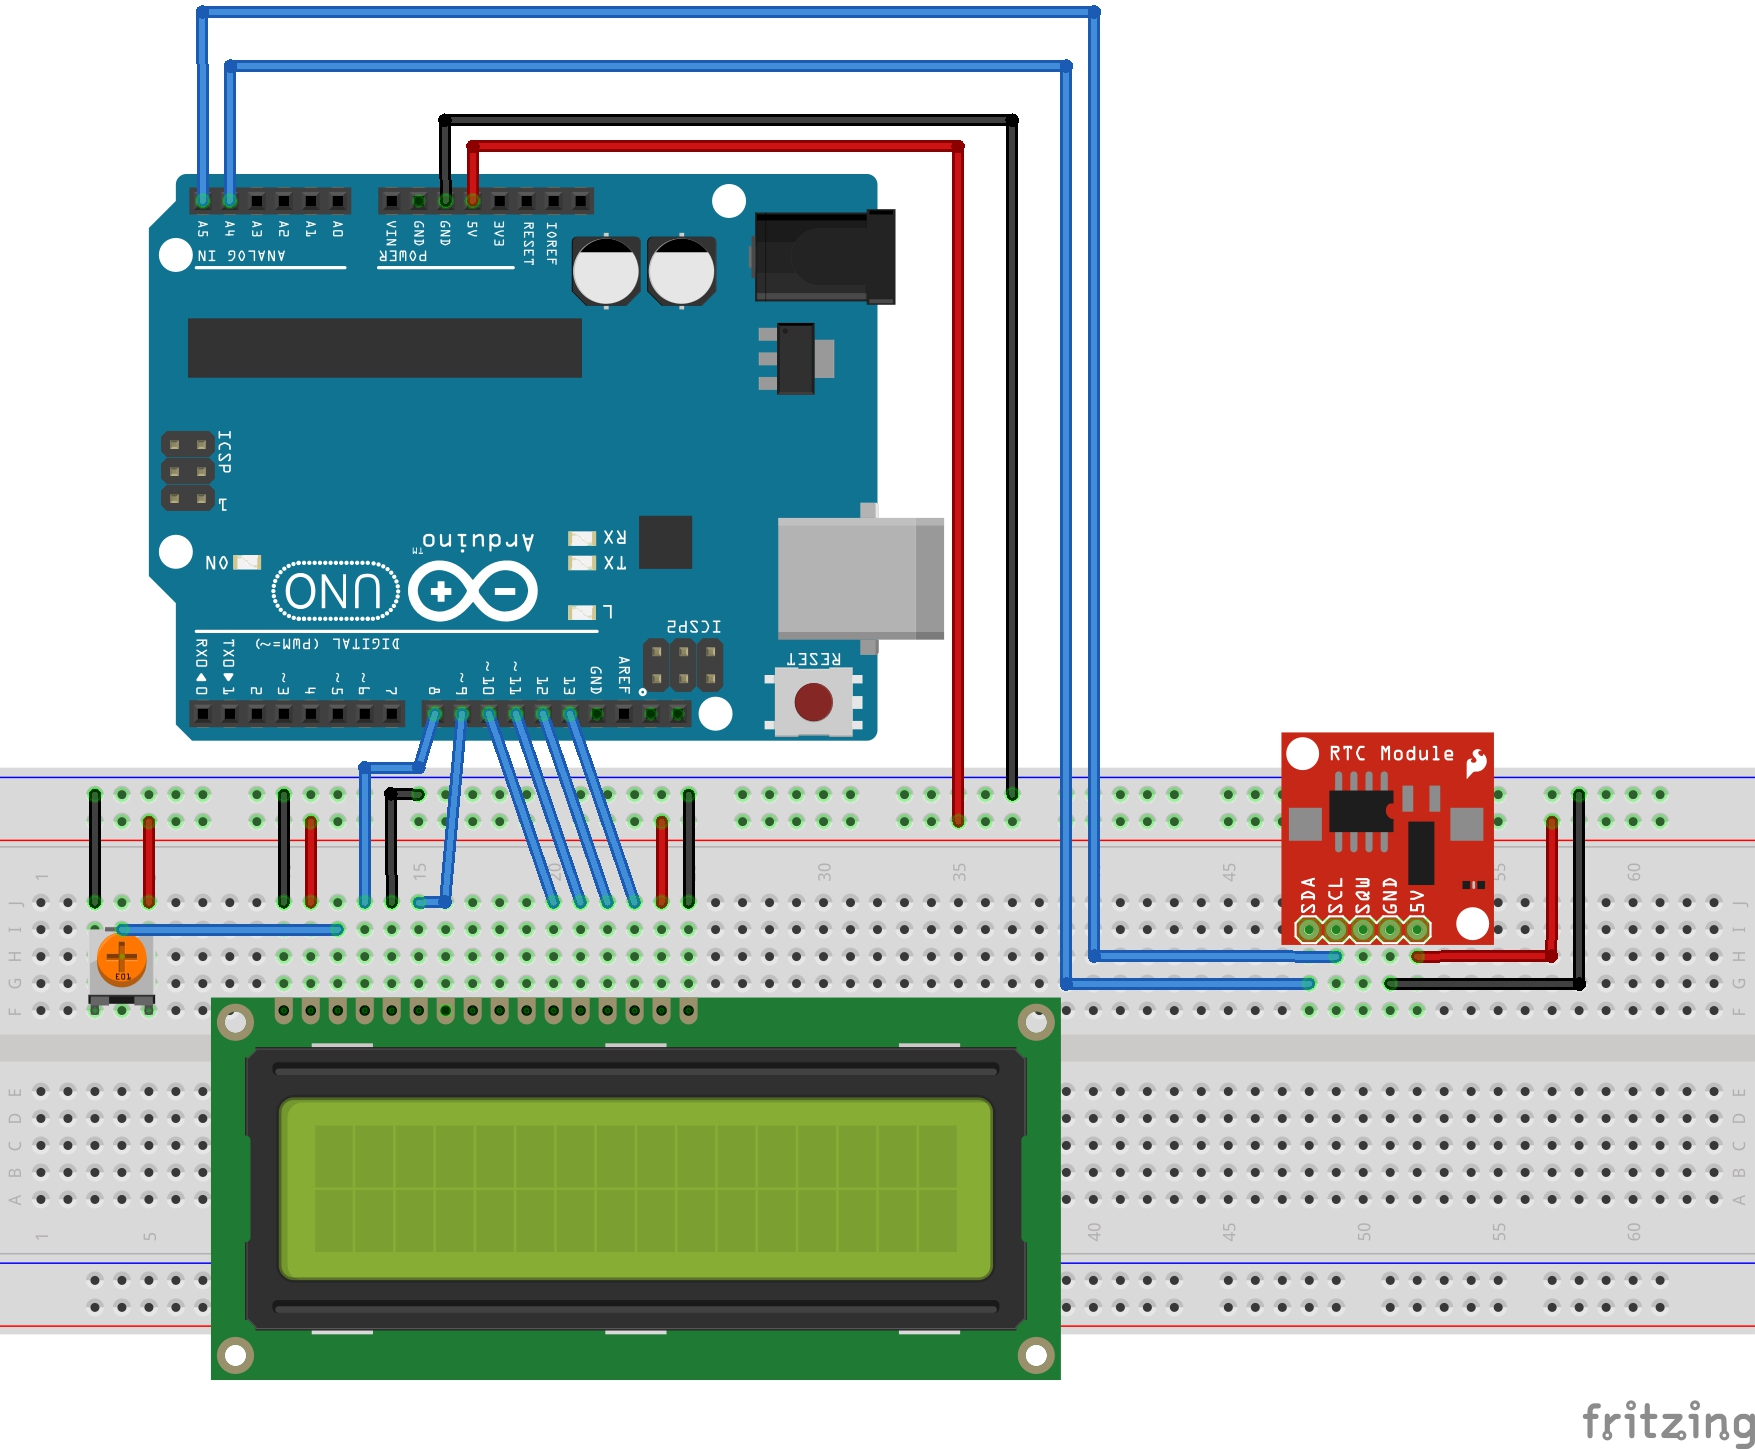
\includegraphics[scale=0.4]{3D.jpg}
\end{figure}

\section{Análisis de Resultados}
\begin{figure}[hbtp]
\caption{Captura del codigo}
\centering
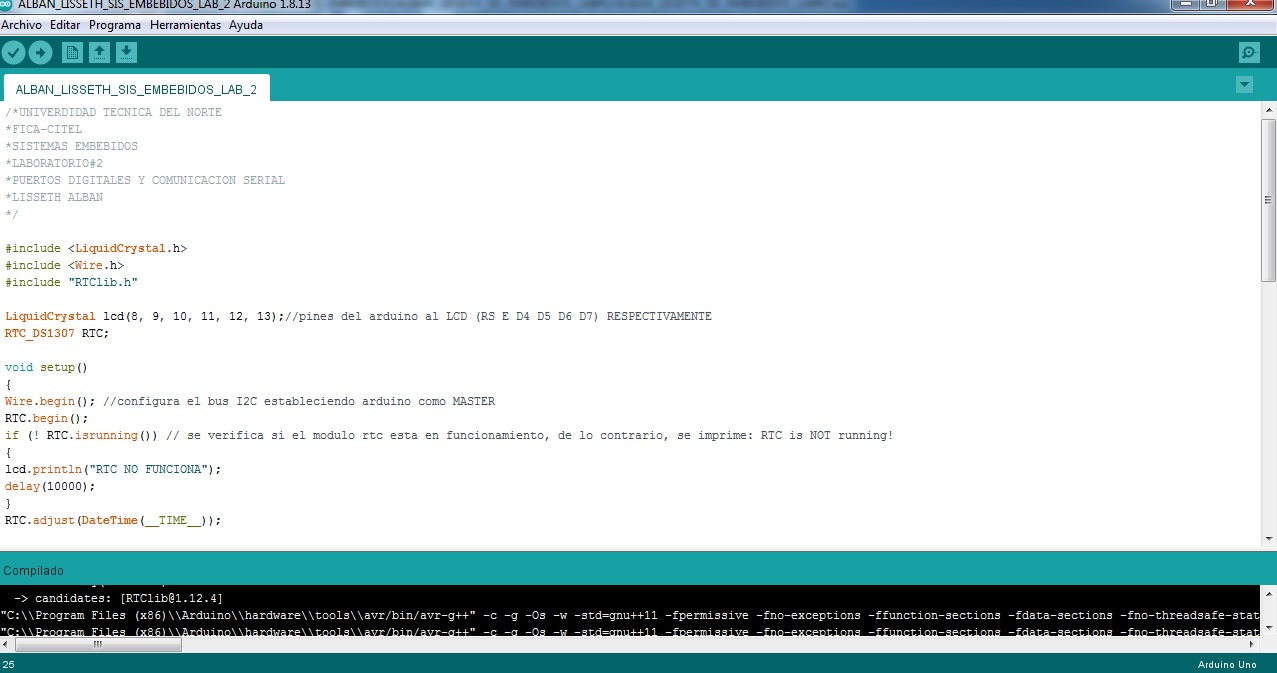
\includegraphics[scale=0.3]{ARDUINO.jpg}
\end{figure}
\begin{figure}[hbtp]
\caption{Captura del codigo}
\centering
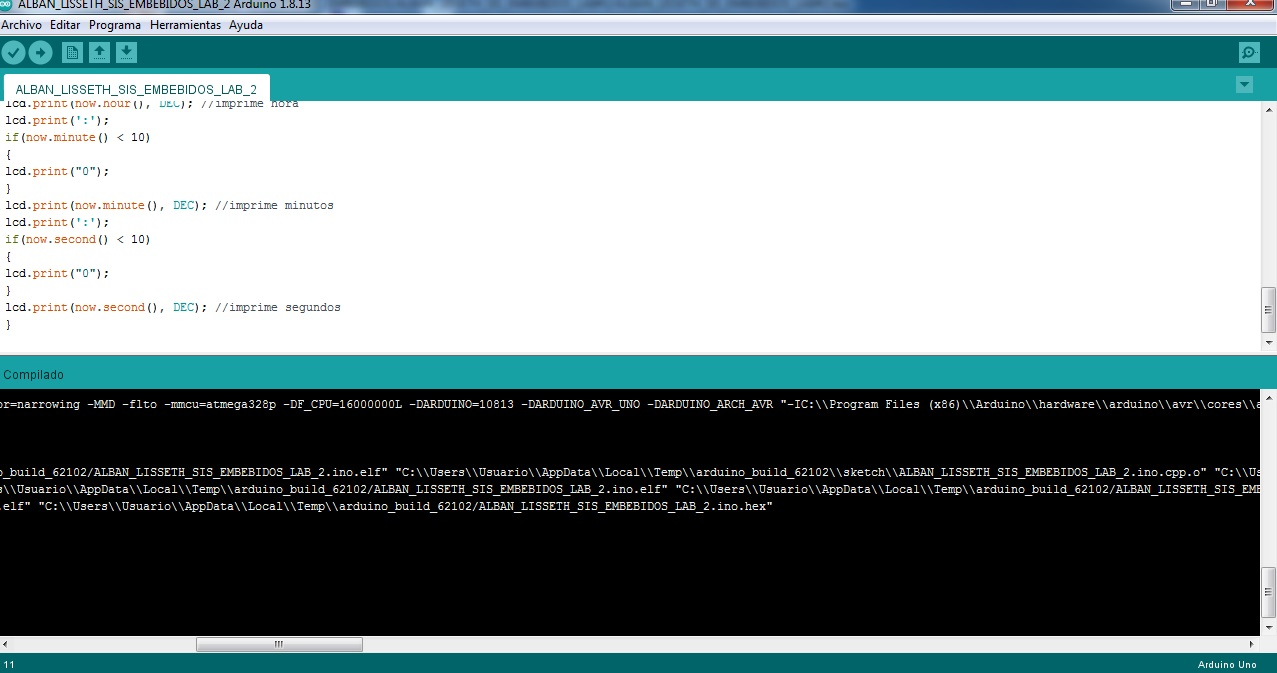
\includegraphics[scale=0.3]{ARDUINO1.jpg}
\end{figure}

\section{Conclusiones y Recomendaciones}
\subsection{Conclusiones}
\begin{itemize}
\item Para la realizacion del laboratorio es necesario revisar que todas la biblitecas que se van a necesitar esten integradas al programa para evitar complicaciones en el momento de desarrollar la aplicacion.
\end{itemize}
\\
\subsection{Recomenciones}
\begin{itemize}
\item Tener muy en cuenta que los programas que se van a usar esten en correcto funcionamiento, y si es necesario revisar tutoriales para evitar confuciones a la ahora de realizar las practicas.
\item Saber representar la lógica de programación al sistema de simulación esto hará́ que se facilite los procesos al momento de crear nuestro circuito.
\end{itemize}
\end{document}